\section{Příklad 2}
% Jako parametr zadejte skupinu (A-H)
\druhyZadani{E}

\large{\textbf{Řešení:}}

%%% Krok 1 - Odstavení zátěže
\begin{center}
    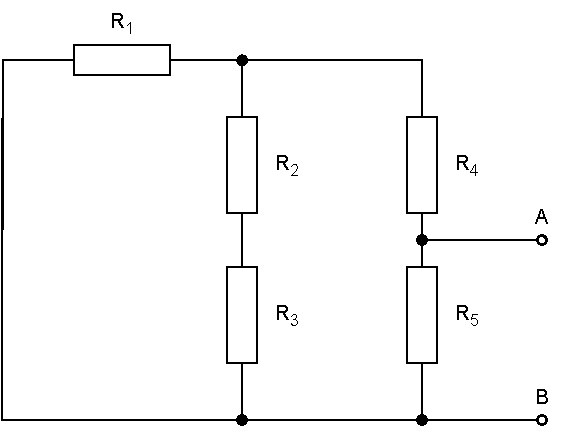
\includegraphics[scale=0.8,keepaspectratio]{fig/solutions/02-sol/02-step1.pdf} \\
    Obr.2.1 Výpočet vnitřního odporu $R_i$, odstraníme zatížení ($R_6$) a zkratujme zdroj.
\end{center}

\begin{gather*}
    R_{23} = R_2 + R_3 = 335 + 625 = 960 \Omega \\\\
    R_{123} = \frac{R_1 \times R_{23}}{R_1 + R_{23}} =
    \frac{150 \times 960}{150 + 960} =
    129.72972973 \Omega \\\\
    R_{1234} = R_{123} + R_4 = 129.72972973 + 245 = 374.72972973 \Omega \\\\
    R_i = \frac{R_{1234} \times R_5}{R_{1234} + R_5} =
    \frac{374.72972973 \times 600}{374.72972973 + 600} =
    230.66685152 \Omega
\end{gather*}

\newpage

%%% Krok 2 - Výpočet U_i pomocí smyčkových proudů
\begin{center}
    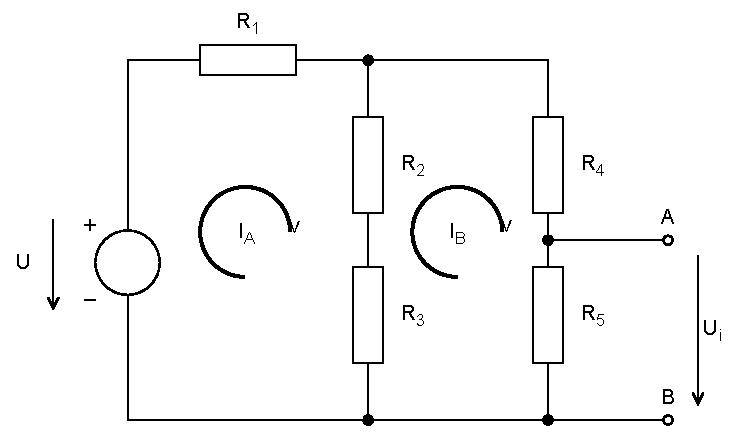
\includegraphics[scale=0.8,keepaspectratio]{fig/solutions/02-sol/02-step2.pdf} \\
    
    Obr.2.2 - Vypočítáme $U_i$ pomocí smyčkových proudů $I_B$
\end{center}

\begin{gather*}
    I_A: I_A(R_1 + R_2 + R_3) + I_B(-R_2 - R_3) = U \\\\
    I_B: I_A(-R_2 - R_3) + I_B(R_2 + R_3 + R_4 + R_5) = 0 \\
\end{gather*}

Převedeme do matice a vypočítáme pomocí Cramerova pravidla
    
\begin{gather*}
    \begin{pmatrix}
    R_1 + R_2 + R_3 & -R_2 - R_3 \\
    -R_2 - R_3 & R_2 + R_3 + R_4 + R_5
    \end{pmatrix}
    \times
    \begin{pmatrix}
    I_A \\
    I_B
    \end{pmatrix}
    =
    \begin{pmatrix}
    U \\
    0
    \end{pmatrix}
\end{gather*}
\\
Vypočítejme determinanty matice
\begin{gather*}
    M =
    \begin{vmatrix}
    1110 & -960 \\
    -960 & 1805
    \end{vmatrix}
    =
    1081950
    \\\\
    M_{I_B} =
    \begin{vmatrix}
    1110 & 250 \\
    -960 & 0
    \end{vmatrix}
    =
    240000
\end{gather*}
\\
Použijeme Cramerovo pravidlo pro výpočet $I_B$:
\begin{gather*}
    I_B = \frac{M_{I_B}}{M} = \frac{240000}{1081950} = 0.22182171 A
    \\\\
    U_i \equiv U_{R_5} = I_B \times R_5 = 0.22182171 \times 600 = 133.09302648 V
\end{gather*}

\newpage

%%% Krok 3 - Pomocí ekvivalentního obvodu vypočítejme I_R6 a U_R6
\begin{center}
    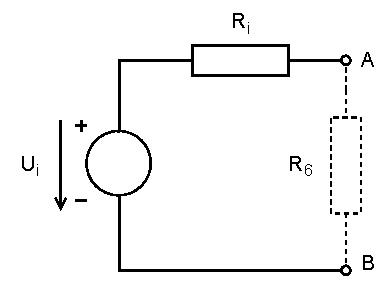
\includegraphics[scale=0.8,keepaspectratio]{fig/solutions/02-sol/02-step3.pdf} \\
    Obr.2.3 - Pomocí ekvivalentního obvodu vypočítejme $I_{R_6}$ a $U_{R_6}$
\end{center}

\begin{gather*}
    \boldsymbol{I_{R_6}} = \frac{U_i}{R_i + R_6} = \frac{133.09302648}{230.66685152 + 300} = \textbf{0.25080335A} \\\\
    \boldsymbol{U_{R_6}} = R_6 \times I_{R_6} = 300 \times 0.25080335 = \textbf{75.24100635V}
\end{gather*}